\documentclass[aip,rsi,reprint,graphicx]{revtex4-1} % for checking your page length
%\\documentclass[aip,rsi,preprint,graphicx]{revtex4-1} % for review purposes
\usepackage{amsmath, amssymb}
%\usepackage[numbers]{natbib}
\usepackage{graphicx}
\begin{document}
\title{An inexpensive vibrating orifice monodisperse droplet generator using a hard
drive actuator arm}
\author{Sebastian Kosch and Nasser Ashgriz}
\email{\{skosch,ashgriz\}@mie.utoronto.ca}
\affiliation{Department of Industrial and Mechanical Engineering, University of
Toronto}
\begin{abstract}
    We propose that the voice coil actuators found in magnetic hard drives are
    fit to supercede loudspeakers as vibration sources in the laboratory setting. A
    specific use case is the excitation of a liquid jet to induce controlled
    breakup into monodisperse droplets. Like speakers, hard drive actuators are cheap and
    ubiquitous, but they are less unwieldy and offer greater amplitudes without
    producing noise. No machining tools or amplifying electronics
    are needed for the construction and operation of the presented droplet generator.
\end{abstract}
\maketitle
\section{Introduction}
The calibration of spray characterization instruments requires a source of
monodisperse droplets. Although drop-on-demand approaches promise
precise control over the droplet generation, their everyday operation poses
challenges (aspired air bubbles, liquid pileups, satellite droplets, etc.).
Consequently, researchers often fall back on continous-stream drop generators
whenever the droplets' exact timing is less important.

Most continuous-stream drop generators are based on the breakup of a liquid jet
into equally-sized, even-spaced droplets when excited with oscillations of an
appropriate frequency. This simple principle has been employed for fifty
years, with orifices typically attached to either one of two vibrating mechanisms: an
ordinary loudspeaker, first employed by Donnelly and Glaberson\cite{Donnelly66}, or a piezoelectric element, as first proposed by Schneider
and Hendricks\cite{Schneider64} and popularized by Berglund and Liu's
design\cite{Berglund73}.

In this paper, we propose a source of oscillation as inexpensive and ubiquitous
as a speaker and as convenient as a piezoelectric element: the actuator arm
found in every magnetic hard drive.
\begin{figure}
\centering
\includegraphics[width=0.42\textwidth]{hdg_images/designpicture.jpg}
\caption{The fully assembled droplet generator. Nozzle is shown as inserted
through actuator arm. \label{fig:photo}}
\end{figure}
%The concept of \emph{on-demand}
%droplet generation is embodied by approaches based on contracting piezoelectric
%elements \cite{Yang97, Ulmke99} or thermal bubble generation \cite{Endo88} -- 
%excellent reviews were published by Le and Lee \cite{Le98, Lee02}. 

%Some of the existing design approaches are \emph{on-demand} generators, which,
%by some precisely controlled mechanism, quickly push a fixed amount of liquid
%out of a small orifice. This category includes designs operating on bending or
%constricting piezoelectric elements \cite{Yang97, Ulmke99} and those based on
%thermoresistors. Excellent reviews are given by \cite{AandB}. While
%drop-on-demand generators are a crucial component in applications like inkjet
%printing or microfluidics, they tend to suffer from aspired air bubbles, pileup
%of liquid around the nozzle tip, clogging, and other issues thwarting reliable
%drop expulsion unless manufactured and operated with great attention to detail.
%
%The alternative to on-demand drop generation is continuous drop generation,
%typically achieved by exciting a liquid jet into regular breakup, although other
%approaches have been proposed \cite{aerodynamic, turningplate}. These
%generators are typically used to calibrate spray characterization devices or to
%study drop coalescence \cite{reddropletbook}.

%The simple principle of breaking up a vertical liquid jet into droplets by means of
%vibration has been employed for many decades. In most laboratories, two
%mechanisms have enjoyed a monopoly on the oscillation part: the ordinary
%loudspeaker, first employed by \citet{Donnelly66}, and piezo elements, as
%popularized by \citet{Berglund73}.

\section{Characteristics}
With high-capacity and solid-state devices rapidly pushing older hard drives
into obsolescence, it should be a simple matter to acquire a few specimens for
demolition. Hard drives come in two form factors---3.5 and 2.5 inches wide,
respectively---and both can be used for the purposes of this paper. 

Unlike loudspeakers, hard drives have a flat base plate which can be drilled
into, allowing for easy installation on any experiment jig. Save for a drill and
a saw, no machining tools are needed for the construction of the droplet
generator.

Like piezoelectric elements, vibrating actuator arms are very quiet, enabling
use at frequencies and amplitudes that would far exceed responsible levels on
a speaker.  In our experiments, the actuator responded to frequencies throughout
our hearing range---i.e., up to $17\,$kHz---and likely well beyond, though we
have not tested the full response range for any given amplitude.

As an added advantage over other designs, no amplification is needed. Below
$100\,$Hz, amplitudes on the order of $0.5\,$cm are easily achieved (albeit they
are of course not needed for droplet production) when a peak-to-peak voltage of
$2-4\,$V is applied. The movement scales down with the inverse of the frequency,
however, such that amplitudes are much smaller at typical operating frequencies
($0.5-10\,$kHz). Nevertheless, the voltages required are well within the ability
of any standard laboratory function generator, and can likely even produced by many
consumer-level computer sound cards.
\begin{figure}
\centering
\includegraphics[width=0.4\textwidth]{hdg_images/needles.png}
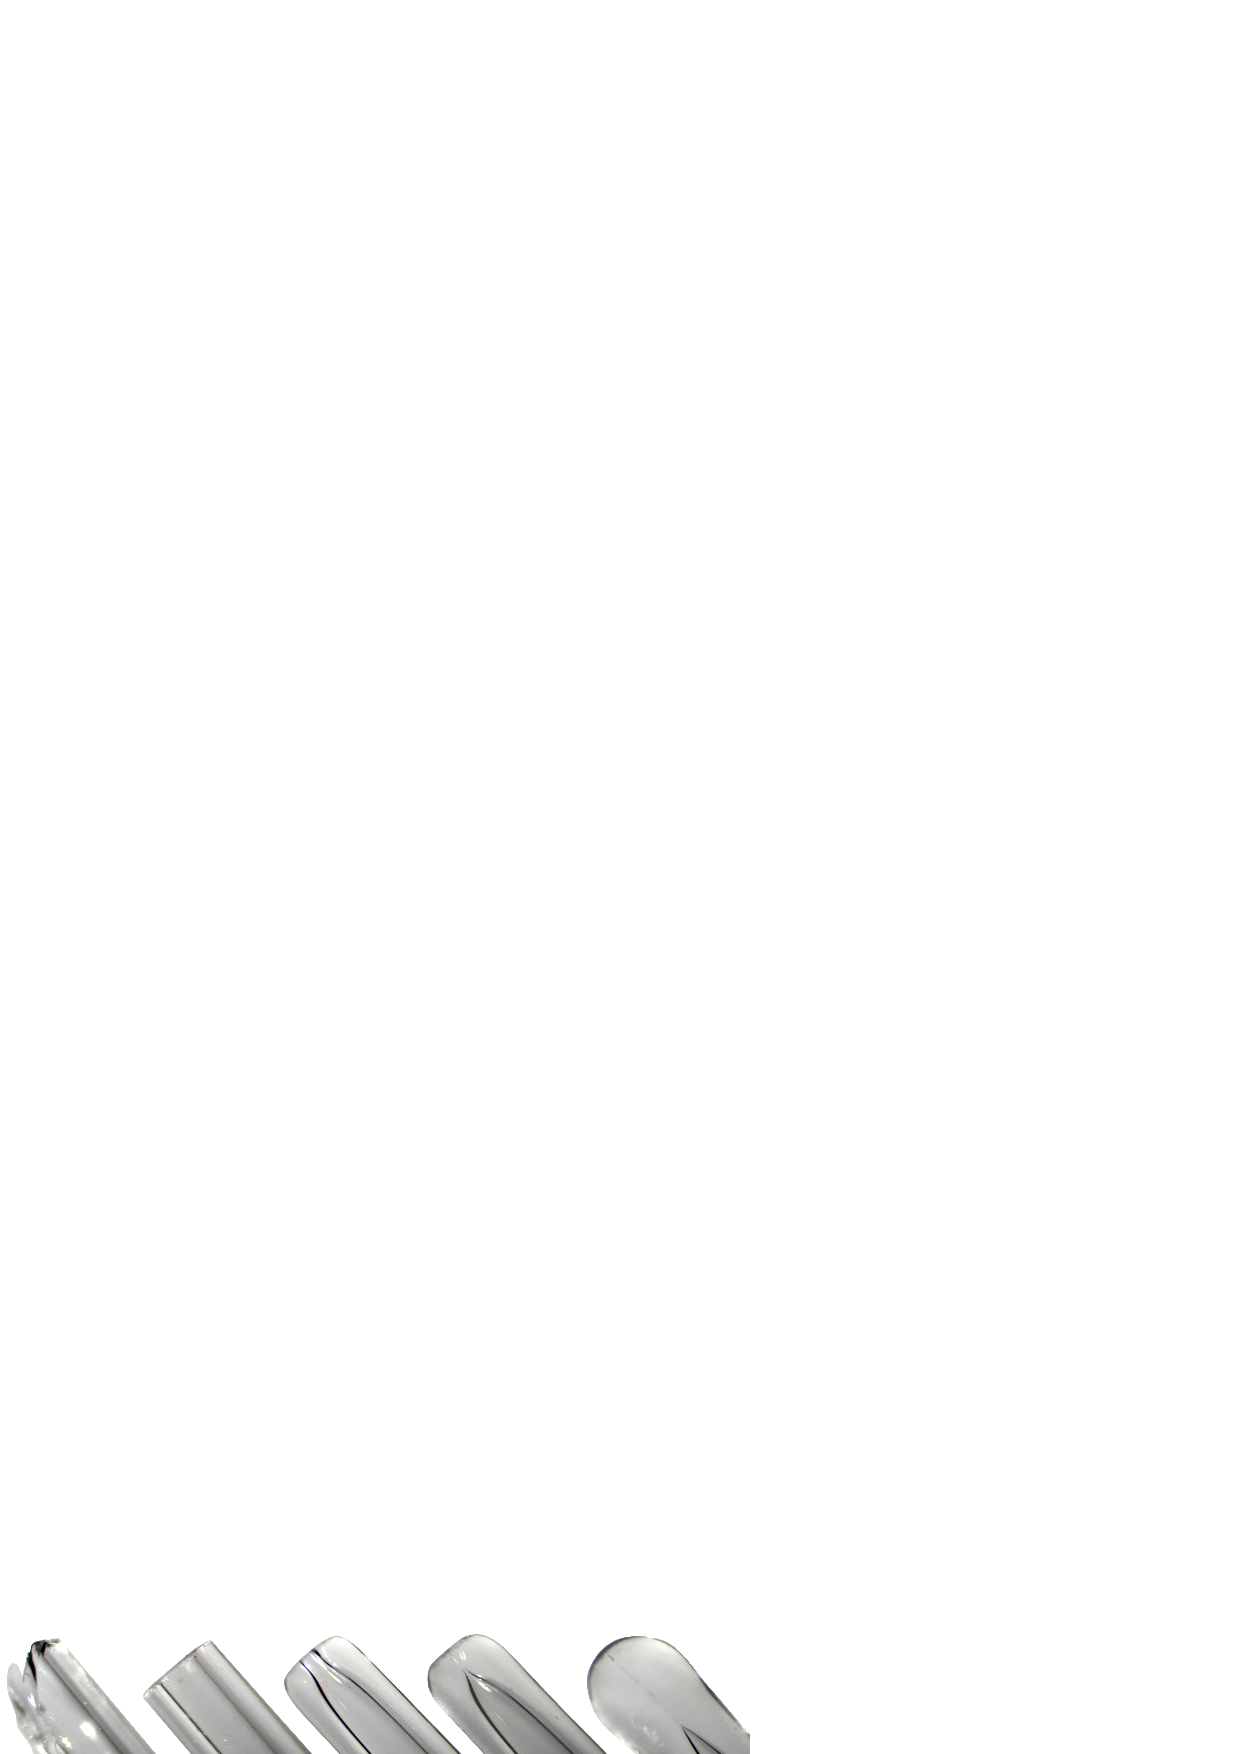
\includegraphics[width=0.35\textwidth]{hdg_images/needletips.png}
\caption{Above: assembly of nozzle from
low-gauge hypodermic syringe (Luer fitting) and capillary. Below: nozzle tip
fabrication, capillary from left to right: broken, sanded, heated in a flame (I.D.
$200\,\mu$m), heated for longer (I.D. $25\,\mu$m, could be sanded down by about
$200\,\mu$m), overheated (I.D. $0\,\mu$m). \label{fig:needles}}
\end{figure}

Finally, glass needle orifices fabricated for use with existing loudspeaker setups can be
reused, and are easily produced by hand from heated borosilicate capillaries or
using a micropipette puller. The process is illustrated in FIG.
\ref{fig:needles} and in-depth instructions are given by Lee\cite{Lee02}.
Piezoelectric-based devices, on the other hand, need fitted orifices to produce a range of
drop sizes.
\section{Construction}
Forgo multi-platter drives, as they are cumbersome to disassemble and have
bulky, complex actuator assemblies. The device shown in FIG. \ref{fig:photo}
is based on a single-platter drive.

\paragraph{Dismantle and cut.} After removing the hard drive cover, remove
the magnet holder, arm axis, arm, ribbon wires, circuit boards, and platters
such that only the base plate remains. Now the corner of the base plate holding
the actuator arm assembly can be cut out to yield the result shown in FIG.
\ref{fig:designschematic}. A band saw, jigsaw or powered hacksaw will be very
useful, although not necessary.

\paragraph{Expose coil leads.} Next, remove the read/write head and all
circuitry leading to it. It can be difficult to discriminate between wiring
connected to the drive's I/O electronics and the two strands powering the voice
coil---we are interested only in the latter, and must be careful not to damage
them. Finally, replace the actuator arm, axis and magnet assembly.
\begin{figure}
\centering
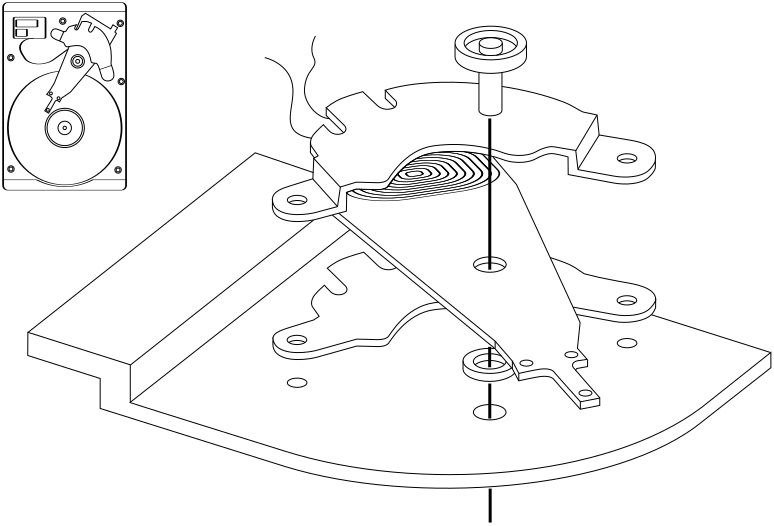
\includegraphics[width=0.4\textwidth]{hdg_images/dropletgenerator_exploded.pdf}
\caption{Top view of a hard drive and exploded view of the cut-out base
plate, actuator arm, axis, and magnet assembly. \label{fig:designschematic}}
\end{figure}
\paragraph{Add protective cover.} We recommend bolting on a cover plate, such
as a small sheet of acrylic or polycarbonate, to protect the protruding arm from
accidental bending. Drill a hole through the cover to allow the nozzle to be
threaded through the arm. A severable
connection from coil to function generator is preferable to a direct wire, if
only because the voice coil leads are delicate and easily torn off. To this end, we epoxied
an audio jack into the cover and soldered the voice coil leads to it from the
bottom. 

\section{Operation} How the nozzle can be held in place falls beyond the scope of
this article; we note that the interchangeability of nozzles with Luer fittings
has proved very convenient in our application. The nozzle must be connected to
an accurately calibrated syringe pump. If a water supply line is integrated into
the setup via a T-valve between pump and nozzle, ensure that it is shut closed
before operation since pressure fluctuations at the nozzle are the most common
culprit for unstable droplet generation.

As with other vibrating orifice droplet generators, it is crucial that stable
conditions are established before any experiments can begin. First, ensure that
the liquid is ejected in a single jet. Multiple jets can be due to a clogged
orifice (a mixture of distilled water and CLR$\circledR$, drawn back through a
syringe, is an excellent remedy). Satellite droplets can also form secondary
jets, in which case the oscillation frequency must be adjusted or the amplitude
reduced. Satellite
formation is easily detected by using a gentle air flow to deflect the jet---if
the droplets are truly monodisperse, they will all deflect at the same
angle.\cite{Strom69}

Note also that the orifice diameter $D_o$ dictates that the range of viable
frequencies $f$ as $3.5 \lesssim \frac{Q}{\pi f \left(\frac{D_o}{2}\right)^2}
\lesssim 7$, where $Q$ is the flow rate). \cite{Savart33, Rayleigh79} In
practice, $D_o$ need not be
precisely determined; it is easy to find appropriate settings for $Q$
and $f$ by viewing the jet against a strobe light, adjusting flow rate for a breakup
length on the order of $10 D_o$ (empirically for water), then tuning the frequency
until droplets appear evenly spaced and spherical.

Under stable conditions, every oscillation of the nozzle will produce one droplet
downstream,\cite{Rayleigh79} such that the droplet diameter will be $D_d = \sqrt[3]{6Q/(\pi f)}$.

\bibliography{hdgbibliography}
\end{document}
